\documentclass[10pt,a4paper]{article}
\usepackage{graphicx}
\usepackage{float}
\usepackage{fullpage}

\begin{document}
\title{Lab 1: Interfacing with the WiiMote}
\author{Sam Mansfield and Toan Vuong \\
  EECS149}
\date{September 11th, 2013}
\maketitle

\section*{Introduction}
  This lab is firstly an introduction to the tools and equipments we'll be using for the class. It identifies skills we should be familiar with, such as scanning manuals for important information and guides. It is also to get us familiarized with interfacing with a WiiMote via bluetooth through LabView, as well as give us a level of expectation for the types of data we can get from the WiiMote.
\section*{Analysis}
  \subsection*{2 Pair a desktop computer with the WiiMote}
    \subsubsection*{a What is the MAC address of your WiiMote?}
      Unfortunately we forgot to write down the MAC address of our WiiMote. It should be in the form AB:CD:EF:GH. Ours was Edward's personal WiiMote.
    \begin{figure}[H]
        \centering
        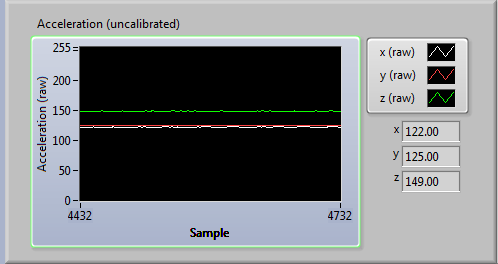
\includegraphics{../lab1_data/lab1_3a.PNG}
        \caption{Uncalibrated acceleration for Question 3}
    \end{figure}
  \subsection*{3 Plot the uncalibrated accelerometer signal from the WiiMote} 
    \subsubsection*{a What are the values of the x and y axes when the WiiMote is at rest on level ground?}
    When the WiiMote is at rest, the x and y axes are at roughly 122 and 125 acceleration, raw.
    \subsubsection*{b What is the value of the z axis when the WiiMote is at rest on level ground? What quantity is begin measured?}
    When the WiiMote is at rest, the z-axis is about 149 acceleration, raw. This is the raw value of gravity that we get from the WiiMote.
  \subsection*{4 Control the WiiMote actuators}
    \begin{figure}[H]
        \centering
        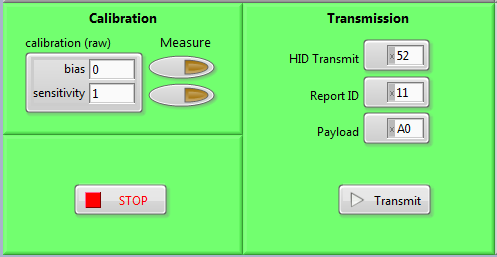
\includegraphics{../lab1_data/lab1_4a.PNG}
        \caption{Transmission data for Question 4a}
    \end{figure}
    \subsubsection*{a What is the Report ID and Payload to turn WiiMote LEDs 2 and 4 on, and LEDs 1 and 3 off?}
    To turn the WiiMote LEDs 2 and 4 on, leaving LEDs 1 and 3 off, we transmit the following packet:
    \begin{tabular}{l | r}
        \textbf{Transaction Header}         & 52 \\
        \hline
        \textbf{Report ID}                  & 11 \\
        \hline
        \textbf{Payload}                    & A0 \\
    \end{tabular}
    \begin{figure}[H]
        \centering
        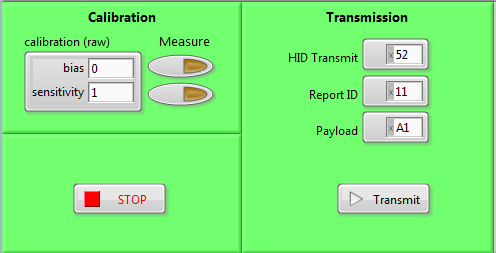
\includegraphics{../lab1_data/lab1_4b.PNG}
        \caption{Transmission data for Question 4b}
    \end{figure}
    \subsubsection*{b How can you modify the above sequence to also enable the rumble motor?}
    We merely add the rumble mask, which is the first bit, to the existing mask in (4a) to enable rumble:
    \begin{tabular}{l | r}
        \textbf{Transaction Header}         & 52 \\
        \hline
        \textbf{Report ID}                  & 11 \\
        \hline
        \textbf{Payload}                    & A1 \\
    \end{tabular}
  \subsection*{5 Measure sensitivity and bias of the accelerometer}
    \begin{figure}[h]
        \centering
        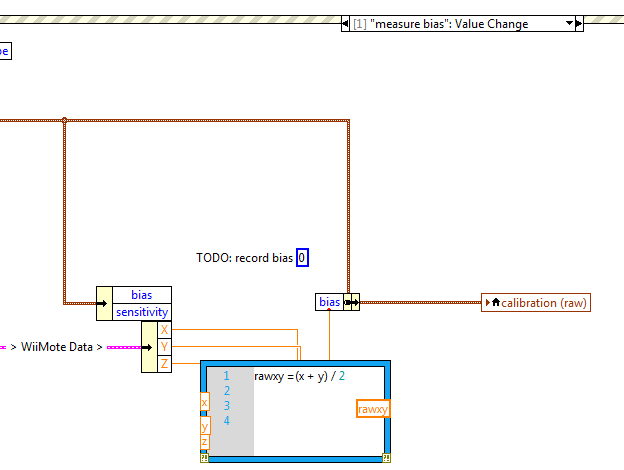
\includegraphics[scale=0.4]{../lab1_data/lab1_5b.PNG}
        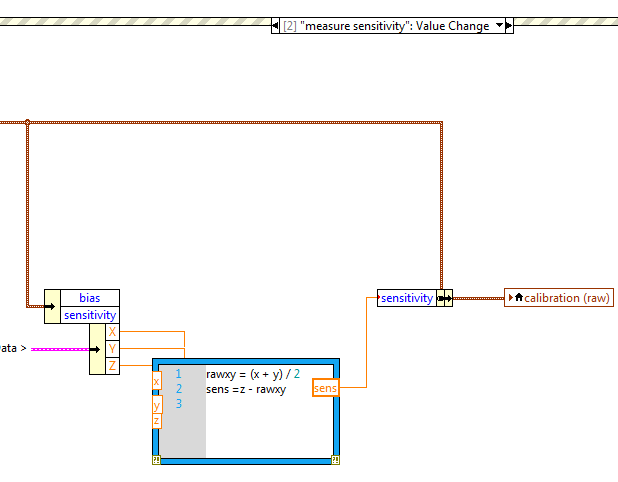
\includegraphics[scale=0.4]{../lab1_data/lab1_5c.PNG}
        \caption{Location of "measure bias" and "measure sensitivity." Note the drop down near the top.}
    \end{figure}
    \subsubsection*{a Where are these measurements stored?}
    These measurements are stored in a subdiagram of the Event Structure. We can access them via \\
    the middle drop down labeled "measure bias" and "measure sensitivity"
    \subsubsection*{b What bias did you record?}
    By taking the average of $\frac{raw_{x} + raw_{y}}{2}$, we got a bias of $124$. 
    \subsubsection*{c What sensitivity did you record?}
    Sensitivity was calculated by the difference $z - bias$, yielding a value of $26$.
    \subsubsection*{d Provide screenshots of changes to the block diagram code}
    See Figure 4 for the screenshots. Both formulas come from the affine model:
    \begin{eqnarray}
        f(x) = ax + b \\
           => x = \frac{f(x) - b}{a}
    \end{eqnarray}
    Letting $b$ be our bias, $f(x)$ be our raw acceleration, $a$ be our sensitivity, we can derive the bias and sensitivity equalities by allowing $x = 1\ g$ when $f(x) = raw_{z}$ (This gives us the sensitivity equation). 
    \begin{eqnarray}
        1 &=& \frac{raw_{z} - bias}{sensitivity} \\
        sensitivity &=& raw_{z} - bias
    \end{eqnarray}
    We also restrict $x = 0$ when $f(x) = raw_{x} = raw_{y}$ (Giving us bias). We average $raw_{x}$ and $raw_{y}$ to get a more accurate bias, $raw_{xy}$. 
    \begin{eqnarray}
        0 &=& \frac{raw_{xy} - bias}{sensitivity} \\
        % Total hack here
        bias &=& raw_{xy}  \ \ \ \ \ \ \ \ \ \ \ \ \ \ \ \ \ \ \ \ \ \ \ \ Assuming\ sensitivity \neq 0
    \end{eqnarray}

  \subsection*{6 Calibrate the accelerometer}
    \subsubsection*{a What equations did you use to calibrate the accelerometer and to calculate the magnitude of the acceleration it measures?}
      To calibrate the accelerometer we used a simple affine function and the assumptions that when the WiiMote is at rest, with the buttons facing upwards, the callibrated x and y will be 0 and the callibrated z will be 1: 
        \[callibratedX = \frac{x - bias}{sensitivity}\] 
        \[callibratedY = \frac{y - bias}{sensitivity}\] 
        \[callibratedZ = \frac{z - bias}{sensitivity}\] 
      And at rest:
        \[callibratedX = \frac{x - bias}{sensitivity} = 0\] 
        \[callibratedY = \frac{y - bias}{sensitivity} = 0\] 
        \[callibratedZ = \frac{z - bias}{sensitivity} = 1\] 
      So solving for bias we get:
        \[bias = x\]
        \[bias = y\]
      And since x and y aren't the same value at rest we averaged x and y for the bias:
        \[bias = \frac{x + y}{2}\]
      To calculate sensitivity we used the following formula:
        \[sensitivity = z - bias\]
      Substituting in bias we get:
        \[sensitivity = z - \frac{x + y}{2}\]
      To solve for magnitude we used the distance formula:
        \[magnitude = \sqrt{x^2 + y^2 + z^2}\]
    \subsubsection*{b Based on your calibration parameters and the number of bits of resolution of the WiiMote ADC, and an affine model of the WiiMote accelerometer, what is your estimate of the maximum acceleration that the WiiMote can measure?}
      The maximum acceleration is when x, y, and z are at their max. It appeared that the max uncalllibrated value of x, y, and z was 256, which would be 8 bits. This gives a max callibrated x, y, and z of:
        \[callibratedXMAX = \frac{256 - bias}{sensitivity} = 0\] 
        \[callibratedYMAX = \frac{256 - bias}{sensitivity} = 0\] 
        \[callibratedZMAX = \frac{256 - bias}{sensitivity} = 1\]
      Substituting in bias and sensitivity:
        \[callibratedXMAX = \frac{256 - 124}{26} \approx 5\] 
        \[callibratedYMAX = \frac{256 - 124}{26} \approx 5\] 
        \[callibratedZMAX = \frac{256 - 124}{26} \approx 5\]
    \subsubsection*{c When the WiiMote is at rest, what should be the value of the magnitude indicator?}
      At rest the only acceleration is gravity. Since we are measuring magnitude in g-forces, it should be 1g. 
    \subsubsection*{d Why is it better to perform calibration at runtime, rather than hard-coding values for the sensitivity and bias of the sensor?}
      The problem with hardcoding values for bias and sensitivity is that you are assuming that the WiiMote will always produce the same uncallibrated values for x, y, and z, which is not a stable assumption. The uncallibrated values can be dependent on temperature, which WiiMote you are using, and age of the WiiMote. 
    \subsubsection*{e Provide the relevant MathScript code and screenshots of changes (if any) to the block diagram}
    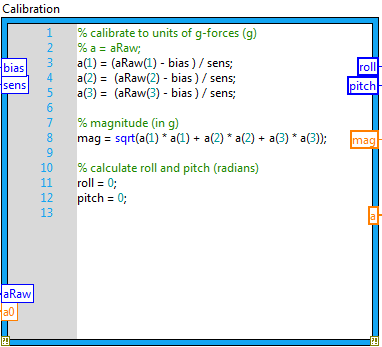
\includegraphics{../lab1_data/lab1_6e.PNG} 
  \subsection*{7 Measure Pitch and Roll}
    \subsubsection*{a What equations did you use to calculate pitch and roll?}
      We used these two equations to calculate pitch and roll:
        \[pitch = \arctan(\frac{y}{\sqrt{x^2 + z^3}})\]
        \[roll = \arctan(\frac{-x}{z})\]
    \subsubsection*{b Provide the relevant MathScript code and screenshots of changes (if any) to the block diagram.}
    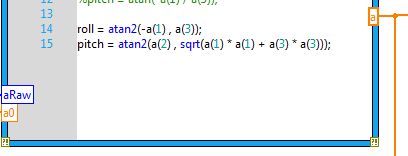
\includegraphics{../lab1_data/lab1_7a.PNG} \\[1em] 
    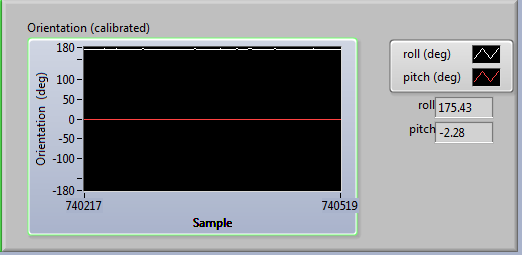
\includegraphics{../lab1_data/lab1_7b.PNG} 
  \subsection*{8 Filter the accelerometer signal}
    \subsubsection*{a Describe your filter, and include an equation for its impulse response, frequency response, or its output as a fraction of input.}
      We used a averaging low pass filter of the form:
        \[Filter(x) = (1 - \alpha)*callibratedX(x) + \alpha*callibratedX(x-1)\]
        \[Filter(y) = (1 - \alpha)*callibratedY(y) + \alpha*callibratedY(y-1)\]
        \[Filter(z) = (1 - \alpha)*callibratedZ(z) + \alpha*callibratedZ(z-1)\]
      We varied the $\alpha$ from 0.5 to 0.99 and decided that 0.9 provided the best response. The signal was less noisy and the delay was still low. This was a good compromise. 
      The impulse response of our filter was:
        \[h(n) = \alpha^n*u(n)\]
      And our frequency response was:
        \[H(j\omega) = \frac{\alpha}{1 - (1 - \alpha)e^{-j\omega}}\]
    \subsubsection*{b Provide the relevant MathScript code and screenshots of changes (if any) to the block diagram}
      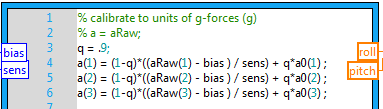
\includegraphics{../lab1_data/lab1_8a.PNG} 
  \subsection*{9 Share Your Feedback}
    This was an overall straightforward and helpful lab to get us started.
\section*{Conclusion}
  This lab helped us to go through the process of receiving unfiltered data from a standard embedded system (WiiMote), and using that data to produce meaningful data, such as a callibrated accelerometer with magnitude. It was helpful to go through the process of figuring out how to calculate the bias and sensitivity without hardcoding the values, which is an extremely good way to think about calibration. It would have been nice to do a little more interfacing with the WiiMote, such as with the turning on and off different features and looking how the data is coming in byte wise and filtering it based on its significance.
  
  Overall the lab covered a broad range of ideas from basic algebra (calculating bias and sensitivity), vector analysis (calculating magnitude, pitch, and roll), and signal analysis (filtering the accelerometer signal). All these skills were simple, but also complicated since we had to pull from different sections of our brain, which was a great exercise. 
\end{document}

